\section{Problem Statement}
\label{sec:intro_problem}

Autonomous VAPT systems face two recurring failure modes that have been independently measured across multiple benchmark studies. The two modes are complementary rather than coincidental: exploration breadth and dependency-aware planning are not separable capabilities. A system that explores widely without a model of which vulnerabilities depend on which others will revisit dead-end paths and waste its iteration budget on routes that are unreachable without prior steps. Conversely, a system that reasons about dependencies only over a pre-supplied weakness set cannot operate on an unfamiliar attack surface where no such set exists in advance. Both quantitative failure modes are described below.

\textbf{Failure Mode 1 --- Insufficient exploration.} On CVE-Bench \citep{zhu2025cvebench}, a benchmark of 40 critical-severity (CVSS $\geq 9.0$) real-world web-application CVEs, the strongest reported agent achieves a pass@5 success rate of only 13\% (one-day setting) and 10\% (zero-day setting). CVE-Bench's failure-mode breakdown (Table~5 of \citealt{zhu2025cvebench}) identifies \emph{insufficient exploration} as the dominant cause of failure across every agent and evaluation setting, with exploration-failure rates ranging from 37.5\% to 80.0\%, as illustrated in Figure~\ref{fig:exploration-failure}. The failure is not merely a matter of insufficient effort: CVE-Bench defines it specifically as an agent's failure to locate the exploitable endpoint, even when given a high-level vulnerability description. Agents converge early on a narrow set of candidate paths and do not return to probe the remainder of the attack surface.

\begin{figure}[htbp]
	\centering
	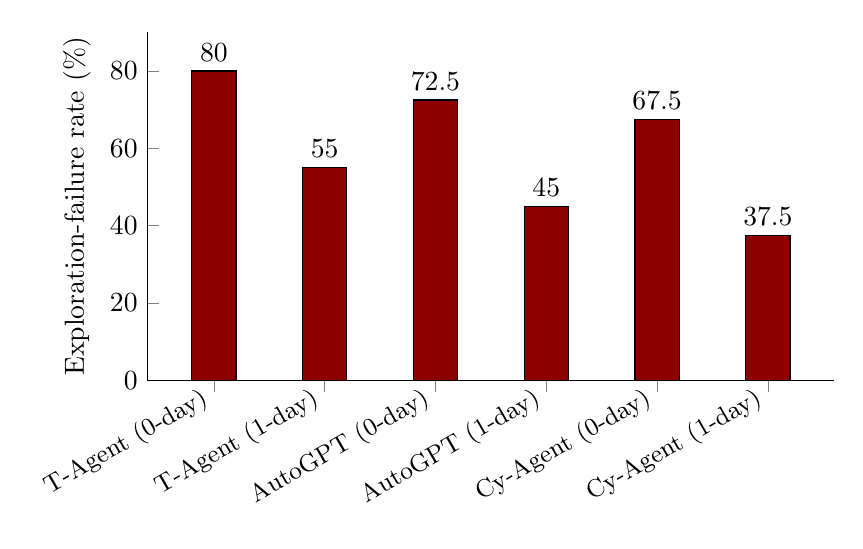
\begin{tikzpicture}
		\begin{axis}[
				ybar,
				bar width=16pt,
				width=0.85\textwidth,
				height=6cm,
				ylabel={Exploration-failure rate (\%)},
				symbolic x coords={T-Agent (0-day),T-Agent (1-day),AutoGPT (0-day),AutoGPT (1-day),Cy-Agent (0-day),Cy-Agent (1-day)},
				xtick=data,
				x tick label style={rotate=30,anchor=east,font=\small},
				nodes near coords,
				nodes near coords align={vertical},
				ymin=0, ymax=90,
				axis lines*=left,
				enlarge x limits=0.12,
			]
			\addplot[fill=red!55!black, draw=black] coordinates {
					(T-Agent (0-day),80.0) (T-Agent (1-day),55.0)
					(AutoGPT (0-day),72.5) (AutoGPT (1-day),45.0)
					(Cy-Agent (0-day),67.5) (Cy-Agent (1-day),37.5)
				};
		\end{axis}
	\end{tikzpicture}
	\caption{Exploration-failure rate as the dominant CVE-Bench failure mode, by agent and evaluation setting. T-Agent is the hierarchical multi-agent framework from \citet{zhu2024hptsa}; data from Table~5 of \citet{zhu2025cvebench}.}
	\label{fig:exploration-failure}
\end{figure}

\textbf{Failure Mode 2 --- The dependency-reasoning gap.} PentestEval \citep{yang2025pentesteval} decomposes the penetration testing pipeline into six sequential stages --- Information Collection (IC), Weakness Gathering (WG), Weakness Filtering (WF), Attack Decision-Making (ADM), Exploit Generation (EG), and Exploit Revision (ER) --- and evaluates nine state-of-the-art LLMs on each. The two weakest stages are WG (average Jaccard similarity 0.29 against expert ground truth) and ADM, the planning stage that requires reasoning about prerequisite relationships between candidate weaknesses. ADM's average Spearman rank correlation against expert judgement is 0.25, consistent across all nine evaluated models (range: 0.07 for GPT-3.5-Turbo to 0.34 for Qwen-Max): no tested model achieves meaningful alignment with expert attack-decision reasoning. The ground-truth-injection ablation in PentestEval quantifies how much end-to-end performance improves when each stage's output is replaced with expert annotations, applied cumulatively, as summarised in Table~\ref{tab:pentesteval-ablation}.

\begin{table}[htbp]
	\centering
	\caption{PentestEval ground-truth-injection ablation: cumulative end-to-end success rate as expert ground truth replaces each stage's LLM output, from left to right \citep{yang2025pentesteval}.}
	\label{tab:pentesteval-ablation}
	\begin{tabular}{@{}lcc@{}}
		\toprule
		\textbf{Configuration}                  & \textbf{End-to-end success} & \textbf{Marginal gain} \\
		\midrule
		SMP (baseline, no ground truth)         & 0.31                        & --                     \\
		\quad + GT Weakness Gathering (WG)      & 0.50                        & +0.19                  \\
		\quad + GT Weakness Filtering (WF)      & 0.53                        & +0.03                  \\
		\quad + GT Attack Decision-Making (ADM) & 0.67                        & \textbf{+0.14}         \\
		\bottomrule
	\end{tabular}
\end{table}

Two observations from Table~\ref{tab:pentesteval-ablation} are critical for motivating this thesis. First, the current end-to-end ceiling without any ground truth is 0.31 --- the SMP baseline that simply executes the five stages in sequence with LLM outputs throughout. Second, ADM delivers the largest single-stage marginal gain (+0.14) of any stage, and this gain is measured on top of an already ground-truthed WG and WF pipeline, not in isolation. The gap between 0.31 and 0.67 --- a 36-point range --- is the portion of end-to-end performance attributable, in this benchmark, to better dependency reasoning alone. Any dynamically constructed dependency structure that an agent builds from its own discovery output, without expert annotation, will approximate rather than match the ground-truth ceiling, so the realistic target sits somewhere within this range rather than at its upper bound.

\textbf{The compound gap.} The two failure modes together identify a gap that appears unaddressed in the reviewed literature. Systems built for broad exploration of an unfamiliar attack surface --- HPTSA \citep{zhu2024hptsa} and VulnBot \citep{kong2025vulnbot} --- dispatch task lists from a central planner without an explicit model of which weaknesses must precede others. The one system in the reviewed literature that models dependencies explicitly --- CHECKMATE \citep{wang2025checkmate}, using PDDL-style planning operators --- requires the operator to enumerate relevant weaknesses before the planning phase begins; it is not designed to operate on an unknown attack surface where no weakness list is available in advance. A third gap is cross-surface evaluability: every system in the reviewed set undergoes evaluation against a single attack-surface family, making it unclear how well any architectural decision generalises beyond the surface on which it was measured.

The problem this thesis investigates is therefore: \textit{can a single LLM-orchestrated multi-agent architecture combine open-ended exploration of an unfamiliar attack surface with a dynamically constructed, prerequisite-aware dependency model, and if so, does the combination produce a measurable improvement in end-to-end task success when evaluated against independently published benchmarks spanning more than one attack-surface family?} Whether this is achievable within the constraints of a six-month research programme, and whether the improvement is large enough to be meaningful, are empirical questions that the remaining chapters describe a plan for answering.
